\documentclass{beamer}

\usetheme{simple}

\usepackage{lmodern}
\usepackage[utf8]{inputenc}
\usepackage{graphicx}
\usepackage{hyperref}
\usepackage{listings}
\usepackage[scale=2]{ccicons}

% TODO: 
%   position adjustement
%   change colours
%       

% Watermark background (simple theme)

\setwatermark{
\includegraphics[height=8cm]{img/docker.png}}


\title{VIRT - Treinamento da Plataforma de Virtualizacao Xen/Docker}
\subtitle{}
\date{\today}
\author{Agnaldo N. Marinho \\ Gabriel Silva}
\institute{\url{http://github.com/agnaldom}}

\begin{document}

\maketitle

\begin{frame}{Docker Containers}
  \framesubtitle{Introdu\c{c}\~ao ao docker}

  \texttt{Docker} \'e uma plataforma aberta, criada com o objetivo de facilitar o desenvolvimento, 
  a implata\c{c}\~ao e a execu\c{c}\~ao de aplica\c{c}\~oes em ambientes isolados. 

  Usando o Docker, voc\^e pode facilmente gerenciar a infraestrutura da aplica\c{c}\~ao, isso agilizar\'a 
  o processo de cria\c{c}\~ao, manuten\c{c}\~ao e modifica\c{c}\~ao do seu servi\c{c}o.
\end{frame}

\begin{frame}{Docker Containers}
    \framesubtitle{Container vs Virtual machines}
    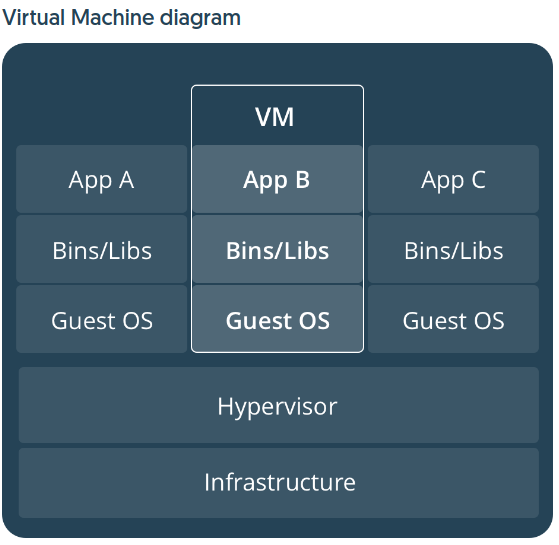
\includegraphics[height=5.7cm]{img/vm.png}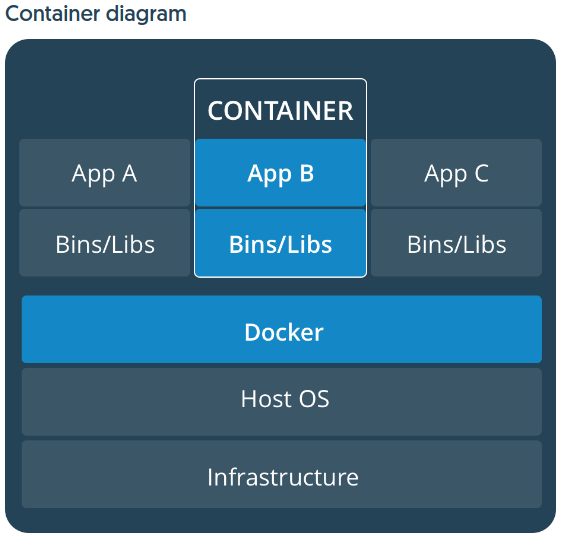
\includegraphics[width=6cm]{img/container.png}
\end{frame}

\begin{frame}{Docker Containers}
    \framesubtitle{Instala\c{c}\~ao Docker}
    \begin{itemize}
        \item Docker est\'a disponivel em duas edi\c{c}\~oes: Community Edition (CE) e Enterprise Edition (EE).
        \item Docker (CE) \'e ideial para desenvolvedores e pequena equipes.
        \item Docker (EE) \'e voltado para times de desenvolvimento e TI das empresas.
    \end{itemize}
    No nosso caso vamos usar o (CE), e para vers\~ao do \href{https://docs.docker.com/engine/installation/linux/docker-ce/debian/}{debian stretch}.
\end{frame}

\begin{frame}{Docker Containers}
    \framesubtitle{Inciando o seu primeiro container}
    Depois da instala\c{c}\~ao, vamos testar a instala\c{c}\~ao rodando o seguinte:
    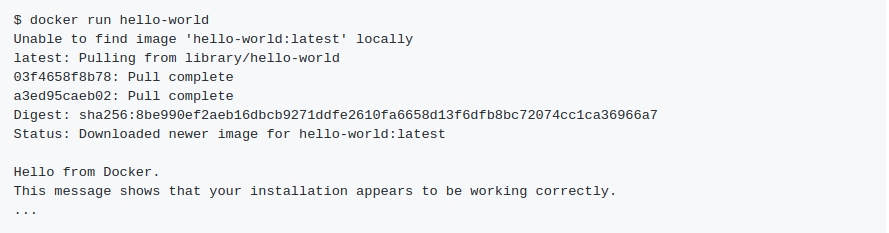
\includegraphics[height=5cm]{img/hello.png}
\end{frame}

\begin{frame}{Docker Containers}
    \framesubtitle{Comandos básicos}
    Para iniciar um container \'e necess\'ario saber a partir de qual imagem será executado. Para lista as
    images que o seu Docker Host tem localmente, execute o comando abaixo>
    \begin{enumerate}
        \item  docker image list
    \end{enumerate}
    Baixando a imagem
    \begin{enumerate}
        \item docker image pull debian
    \end{enumerate}
    Baixamos uma imgem do debian, caso deseje inspecionar a imagem que acabou de atualizar, bastar usar o comando abaixo:
    \begin{enumerate}
        \item docker image inspect debian
    \end{enumerate}
    O comando inspect \'e respons\'avel por informa todos os dados referentes \`a imagem.
\end{frame}

\begin{frame}{Docker Containers}
    \framesubtitle{Criando sua pr\'opria imagem no Docker}
    Uma imagem nada mais \'e do que um ambiente totalmente encapsulado e pronto para ser replicado onde desejar.
    Há duas formas de criar images customizadas: com commit e com Dockerfile.
    \begin{itemize}
        \item Criando images com commit
    \end{itemize}
    Primeiro criamos um container :
    \begin{enumerate}
        \item docker run -it --name dockercurso-debian debian:latest /bin/bash
    \end{enumerate} 
    Agora que estamos no bash do container, instalamos o nginx:
    \begin{enumerate}
        \item apt-get update
        \item apt-get install nginx -y
        \item exit
    \end{enumerate}
    Paramos o container com o comando abaixo:
    \begin{enumerate}
        \item docker container stop dockercurso-debian 
    \end{enumerate}
\end{frame}

\begin{frame}{Docker Containers}
    \framesubtitle{Criando sua pr\'opria imagem no Docker}
    Agora, efetuamos o commit desse container em uma imagem:
    \begin{enumerate}
        \item docker container commit dockercurso-debian dockercurso-nginx
    \end{enumerate}
    Para visualizar a lista de imagens e encontrar a que acabou de criar,
    execute novamente o comando abaixo:
    \begin{enumerate}
        \item docker image list
    \end{enumerate}
    Para testar sua nova image, vamos criar um container a parti dela e verificar se o nginx está instalado:
    \begin{enumerate}
        \item docker run -it --rm dockercurso-nginx dpkg -l nginx
    \end{enumerate}
\end{frame}

\begin{frame}{Docker Containers}
    \framesubtitle{Criando imagens com Dockerfile}
    O docker permite que possamos criar images a partir de um arquivo de defini\c{c}\~ao, 
    esse arquivo chama-se Dockerfile. Em resumo, o Dockerfile  um arquivo texto com
    instru\c{c}~oes, comandos e passos que voc\^e executaria manualmente, basicamente
    o Docker executa uma receita de bolo.
    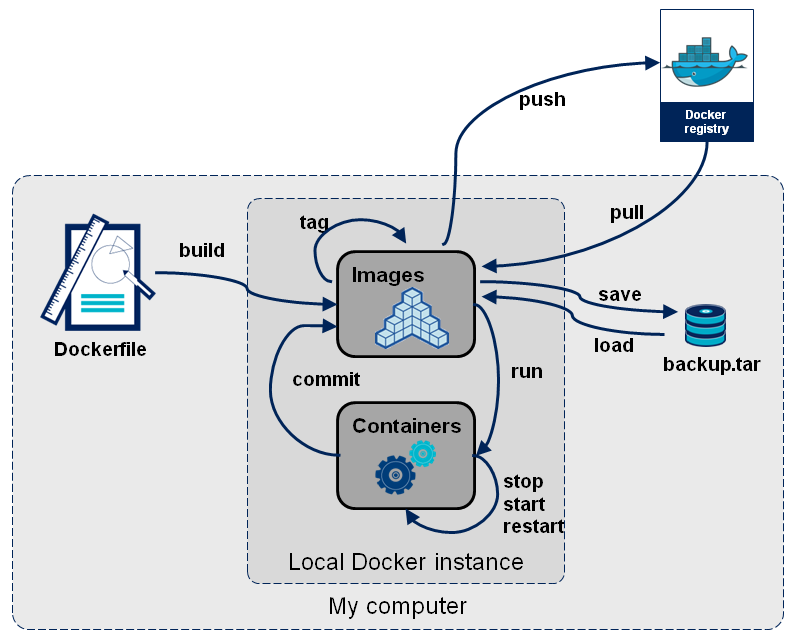
\includegraphics[height=5cm]{img/docker-stages.png}
\end{frame}

\begin{frame}{Docker Containers}
    \framesubtitle{Criando imagens com Dockerfile}
    Atrav\'es do comando docker build, o Docker realizar a execu\c{c}\~ao desses passos 
    e no fina da execu\c{c}\~ao ele encapsula cada layer gerada dentro da imagem.

    O Dockerfile deve seguir uma ordem ou formata\c{c}\~ao correta para que o build
    seja feito de forma certa.

    Exemplo:

    RUN apt-get update

    onde:

    RUN  \'E a instru\c{c}\~ao;

    apt-get update: Argumento que ser\'a executado.

    \href{https://docs.docker.com/engine/reference/builder/}{Dockerfile Referência Oficial}
\end{frame}


\begin{frame}{Docker Containers}
    \framesubtitle{Criando imagens com Dockerfile}
    \href{https://github.com/agnaldom/curso-docker/blob/master/images/nginx/Dockerfile}{
\includegraphics[height=5cm]{img/docker-nginx.png}}
\end{frame}
\begin{frame}{Docker Containers}
    \framesubtitle{Criando imagens com Dockerfile}
    
\includegraphics[height=2cm]{img/docker-php.png}
\end{frame}

\begin{frame}{Docker Containers}
    \framesubtitle{Exporta\c{c}\~ao de containers}
    Imagine que temos um container em execu\c{c}\~ao e queremos export\'a-lo para outro host.

    Podemos criar uma imagem partindo de um container que está funcionando, e gerar um arquivo .tar usando a op\c{c}\~ao save. Como mostrar abaixo:
    \begin{enumerate}
        \item docker ps -q
        \item b02af9430141
        \item docker commit b02af9430141  dockercurso-nginx
        \item 9a8c0a1a72d2f9c2815e455a22be91f9cf788f769d2cca5b603bae
    \end{enumerate}
    De posse da nova imagem que foi gerda.
    \begin{enumerate}
        \item docker save dockercurso-nginx $>$ /tmp/dockercurso-nginx.tar
    \end{enumerate}
    Para fazer a importa\c{c}\~ao desse arquivo, utilizamos a op\c{c}\~ao load.
    \begin{enumerate}
        \item docker load $<$ /tmp/dockercurso-nginx.tar
    \end{enumerate}
\end{frame}

\begin{frame}{Docker Containers}
    \framesubtitle{Gerenciando dados em Docker}
    O Docker oferece tr\^es formas diferentes de montar dados em um container para um Docker Host: Volumes,
    bind mounts, ou tmfs volumes.
        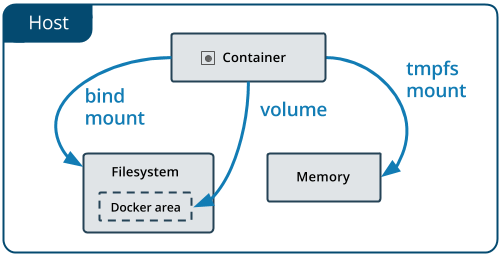
\includegraphics[height=4cm]{img/types-of-mounts.png}
\end{frame}

\begin{frame}{Docker Containers}
    \framesubtitle{Gerenciando dados em Docker}
    \begin{itemize}
        \item Volumes: s\~ao armazenados em uma parte do sistem de arquivos do host que \'e gerenciado pelo docker (/var/lib/docker/volumes/ no linux).
            Os processos n\~ao Docker n\~ao devem modificar esta parte do sistema de arquivos.
        \item Bind Mounts: podem ser armazenadas em qualquer lugar no sistema host. Eles podem at\'e ser importantes arquivos ou diret\'orios do sistema.
            Os processos n\~ao Docker no host ou um cont\^einer Docker podem modific\'a-los a qualquer momento.
        \item tmfs mounts: s\~ao armazenados somente na mem\'oria do sistema host e nunca s\~ao escritas no sistema de arquivos do host.
    \end{itemize}
\end{frame}

\begin{frame}{Docker Containers}
    \framesubtitle{Dados em Docker Volumes}
    Os Volumes  t\^em v\'arias vantagens sobre bind mounts:
    \begin{itemize}
        \item Os volumes s\~ao mas f\'aceis de fazer backup ou migrar do que os bind mounts.
        \item Voc\^e pode gerenciar volumes usando os comando Docker CLI ou a API Docker.
        \item Os volumes funcionam em recipiente Linux e Windows.
        \item Os controladores de volume permitem armazenar volumes em hosts remotos ou provedores
            de nuvem, criptografar o conte\'udo do volumes ou adcionar outros funcionanalidades.
        \item O conte\'udo do um novo volume pode ser pr\'e-preenchido por um container.
    \end{itemize}
    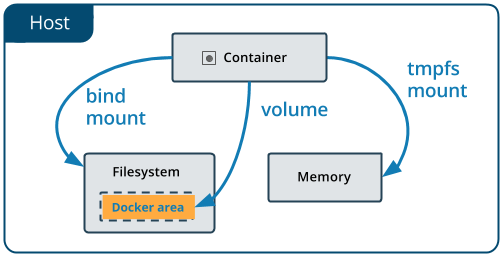
\includegraphics[height=3cm]{img/types-of-mounts-volume.png}
\end{frame}

\begin{frame}{Docker Containers}
    \framesubtitle{Usando Volumes}
    Originalmente, o flag  -v ou --volumes foi usado para cont\^eines independentes e o --mount foi usado para serviços do swarm, 
    a parte da vers\~ao 17.06, voc\^e tamb\'em pode usar --mount para cont\^einer independente.

    Criando volume:
    \begin{enumerate}
        \item  docker volume create site
    \end{enumerate}

    Listando Volumes:

    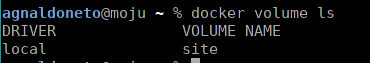
\includegraphics[height=0.8cm]{img/volume-ls.png}

    Inspecionando o volume:

    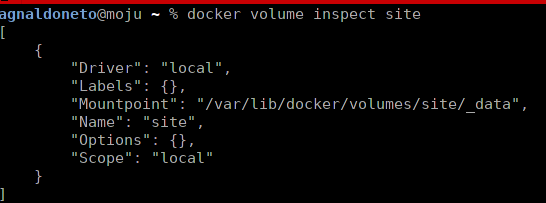
\includegraphics[height=2cm]{img/volume-inspect.png}

    Removendo volume:
    
    docker volume rm site

    \href{https://docs.docker.com/engine/admin/volumes/volumes/}{Documenta\c{c}\~ao Oficial}
\end{frame}

\begin{frame}{Docker Containers}
    \framesubtitle{Docker Compose v3}
    
\includegraphics[height=7.5cm]{img/docker-compose.png}
\end{frame}

\begin{frame}{Docker Containers}
    \framesubtitle{Docker Compose}
    Usar o Compose \'e basicamente um processo de tr\^es passos:
    \begin{enumerate}
        \item Defina o ambiente do seu aplicativo com um Dockerfile para que ele possa ser reproduzido em qualquer lugar.
        \item Defina os servi\c{c}os que comp\~oem seu aplicativo no docker-compose.yml para que eles possam ser executados juntos em ambiente isolado.
        \item Por fim, execute docker-compose up e Compose ir\'a iniciar e executa o aplicativo inteiro.
    \end{enumerate}
\end{frame}

\begin{frame}{Docker Containers}
    \framesubtitle{Docker Compose Joomla}
    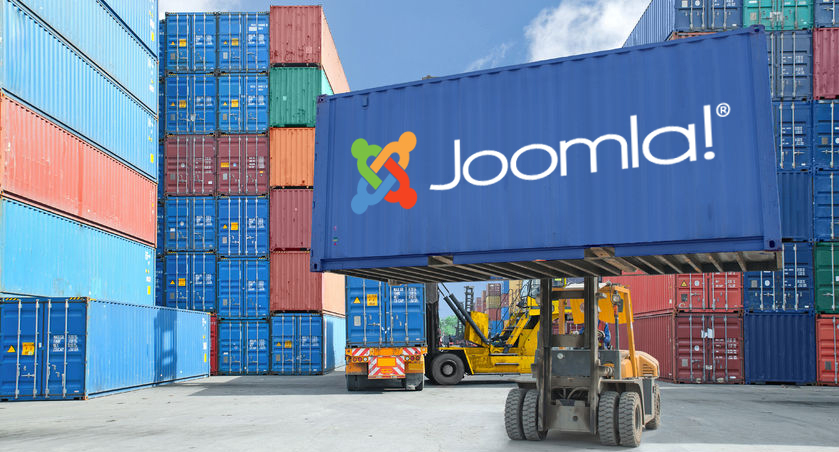
\includegraphics[height=7.5cm]{img/joomla.jpg}
\end{frame}

%\begin{frame}{Docker Containers}
%    \framesubtitle{Docker Compose Joomla}
%    \includegraphics{img/giphy.gif}
    %\end{frame}

\begin{frame}{License}

  \begin{block}{Get the source of this theme and the demo presentation from}

  \begin{center}\url{http://github.com/famuvie/beamerthemesimple}\end{center}

  \end{block}
  
  The theme \emph{itself} is licensed under a
  \href{http://creativecommons.org/licenses/by-sa/4.0/}{Creative Commons
  Attribution-ShareAlike 4.0 International License}.

  \begin{center}\ccbysa\end{center}

\end{frame}

\end{document}

